\section*{Глава 4. Результаты расчётов.}
\addcontentsline{toc}{section}{Глава 4. Результаты расчётов.}
\setcounter{section}{4}
\setcounter{subsection}{0}
\setcounter{equation}{0}

\subsection{Особенности расчёта}

	Основные результаты представленной работы были получены с использованием расчётного модуля, разработанного в ходе выполнения работы. За основную модель была принята модель двухфазной двухкомпонентной неизотермической трёхмерной фильтрации в пласте с ухудшенными ФЕС ОЗП, прошитом системой перфорационных каналов, с фазовыми переходами. За математическую модель принята смешанная задача для системы из двух дифференциальных уравнений\eqref{eqns2}, \eqref{init_cond}, \eqref{well_cond4}, \eqref{well_cond1}, \eqref{well_cond2} либо \eqref{eqns2}, 		\eqref{init_cond}, \eqref{well_cond4}, \eqref{well_cond1}, \eqref{well_cond3} и дифференциального уравнения \eqref{energy_last} c условиями \eqref{energy_init}, \eqref{energy_contour3}, \eqref{energy_contour}, \eqref{energy_contour1} коэффициенты которого определяются решением системы на каждом временном шаге.
	В модели предполагается независимость PVT-свойств флюида и пласта от температуры, также независимость тепловых PVT-свойств от давления.

	Для решение поставленной задачи были использованы численные схемы \eqref{pres_scheme}, \eqref{energy_scheme} метода конечных объёмов для гидродинамической системы и комбинированная схема для уравнения баланса энергии.
	Схема для гидродинамической части задачи была подвергнута линеаризации по Ньютону, решение системы было получено в результате соответствующих итераций.
	Уравнение баланса энергии -- линейно, его решение находилось за одну итерацию.

	Решение задачи производилось последовательно: на кадом шаге по времени решалась итерационно гидродинамическая часть, затем решалось уравнение баланса энергии. В качестве расчётной сетки была выбрана регулярная сетка в цилиндрической системе координат, логарифмически сгущающаяся к скважине.
	Каналы задавались специальными вырезами ячеек, при этом сетка оставалась регулярной.

\subsection{Верификация расчёта}

	Проведённый расчёт был верифицирован с привлечением коммерческого гидродинамического симулятора пласта, всех известных полуаналитических аналитических решений для данной задачи.

	На Рис. \ref{pic:tempest_cmp} представлено сравнение результатов расчётов гидродинамической части задачи.
	Как можно увидеть результаты расчётов написанного модуля полностью совпадают с результатом коммерческого симулятора.
	Использована следующая постановка: двухфазная двухкомпонентная фильтрация с фазовыми переходами, запуск с постоянным дебитом $Q=100 \frac{\text{м}^3}{\text{сут}}$, затем остановка на КВД без ВСС $Q=0 \frac{\text{м}^3}{\text{сут}}$.
\begin{figure}[H]

	\begin{subfigure}[b]{0.5\textwidth}
	\centering
	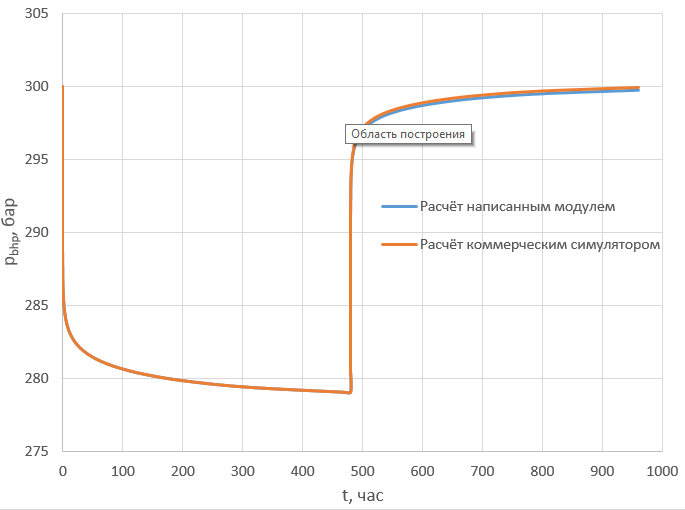
\includegraphics[width=1\textwidth]{pic/pres_cmp.png}
	\caption{Сравнение забойных давлений.}
	\label{pic:pres_cmp}
	\end{subfigure}
~
	\begin{subfigure}[b]{0.5\textwidth}
		\centering
		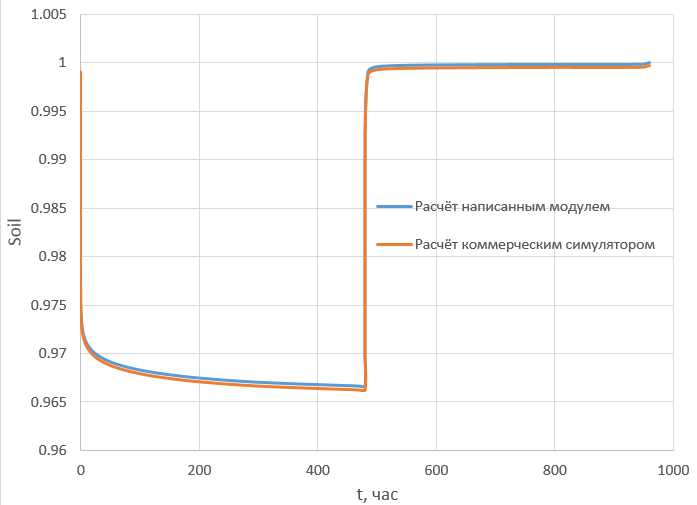
\includegraphics[width=1\textwidth]{pic/sat_cmp.png}
		\caption{Сравнение нефтенасыщенности.}
		\label{pic:sat_cmp}
	\end{subfigure}
	\caption{Сравнение расчёта двухфазной постановки с расчётом коммерческим симулятором. Запуск с постоянным дебитом $Q=100 \frac{\text{м}^3}{\text{сут}}$, затем остановка на КВД без ВСС $Q=0 \frac{\text{м}^3}{\text{сут}}$.}
	\label{pic:tempest_cmp}
\end{figure}

	Выше уже было представлено сравнение расчётов модулем с доступной аналитикой.
	А именно, на Рис. \ref{pic:tunnels} было представлено сравнение расчёта системы перфорационных каналов с указанной аналитикой \cite{tariq}. На Рис. \ref{pic:analytic_cmp} было проиллюстрировано совпадение расчёта забойной температуры модуля с аналитическими выражениями из \cite{checkalyuk}, \cite{ramazanov_spe} в однофазной постановке.
	Также на Рис. \ref{pic:part_pen1}, \ref{pic:part_pen} представлены распределения дебита вдоль ствола скважины, которые также полностью совпадают с расчётом коммерческим симулятором в модели ствола бесконечной проводимости.

	Все вышеуказанные сравнения и примеры, а также многие другие результаты работы указывают на достоверность результатов расчёта разработанного комплекса программ.

\subsection{Вклад различных эффектов в температурную аномалию на забое}
	
	Температурную аномалию на забое составляют следующие эффекты: разнонаправленный эффект Джоуля-Томпсона от нефти и газа, эффект адиабатического расширения нефти и газа, теплота фазового перехода, ковективный и кондуктивный перенос тепла.	Рассмотрим влияние этих эффектов на динамику забойной температуры.

	На Рис. \ref{pic:effects} представлен вклад каждого (кроме теплопроводности, $\tilde{\lambda}=0$) из эффектов в полную температурную аномалию для некоторой синтетической постановки -- выход на режим, затем остановка на КВД.
	Рассмотрим подробно этот пример.
	Из Рис. \ref{pic:effects} видно, что основные эффекты обеспечивающие наибольший вклад в температурную аномалию -- эффект Джоуля-Томпсона нефти, теплота фазового перехода, конвективный перенос тепла (хорошо просматривается на графике полной температуры при остановке скважины).
\begin{figure}[H]
	\centerline{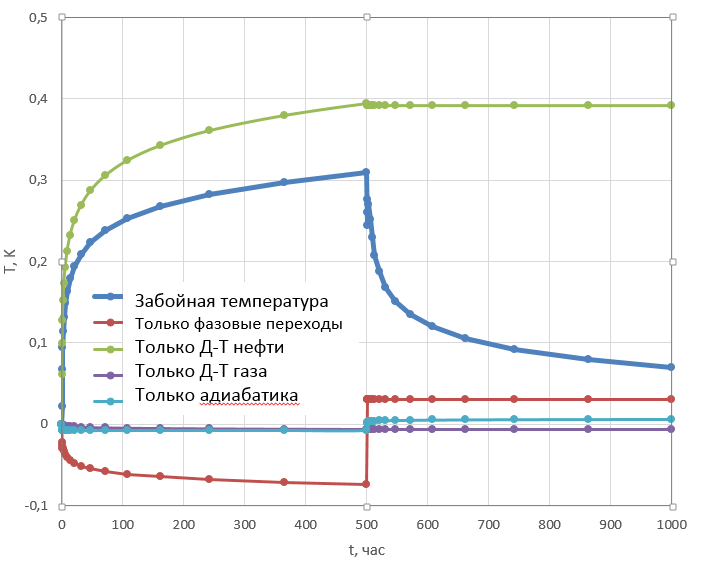
\includegraphics[width=0.6\textwidth]{pic/effects.png}}
	\caption{Вклад различных термодинамических эффектов в температурную аномалию на забое.}
	\label{pic:effects}
\end{figure}

	Все указанные процессы (кроме фазовых переходов) имеют составлющие от жидкой и газовой фаз, которые, в свою очередь, могут вносить вклад в общую температуру с разными знакими. Так, например, известно, что в типичных пластовых условиях коэффициент Джоуля-Томпсона для нефти положителен, а для газа отрицателен. Таким образом, в зависимости от газового фактора, ОФП и PVT хар-к флюидов эф-т Джоуля-Томпсона может приводить как к положительной температурной аномалии, так и к отрицательной. На Рис. \ref{pic:jt_curves} представлены соотвествующие кривые для нескольких значений газового фактора. Расчёты показывают, что отрицательная температурная аномалия может иметь место лишь при огромных значениях газового фактора ($\Gamma \sim 100$), 
на практике такие случаи встречаются редко.
\begin{figure}[H]
	\begin{subfigure}[b]{0.5\textwidth}
	\centering
	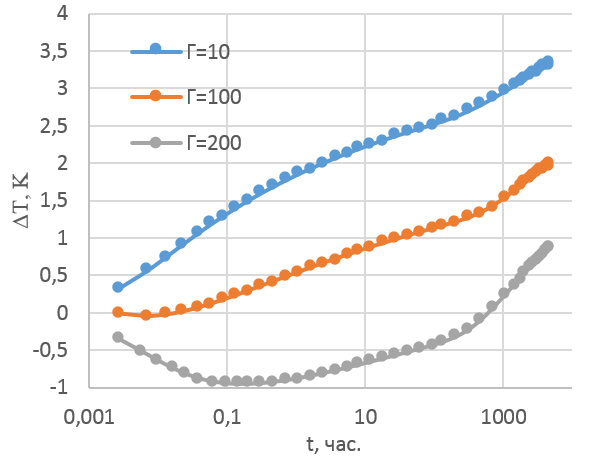
\includegraphics[width=1\textwidth]{pic/gas_factor.png}
	\caption{Температурная аномалия вследствие эффекта Джоуля-Томпсона, при различных газовых факторах нефти.}
	\label{pic:gas_factor}
	\end{subfigure}
~
	\begin{subfigure}[b]{0.5\textwidth}
		\centering
		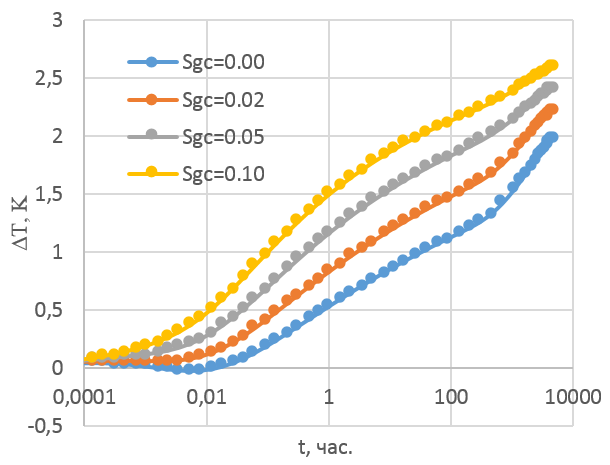
\includegraphics[width=1\textwidth]{pic/critical_gas.png}
		\caption{Температурная аномалия вследствие эффекта Джоуля-Томпсона, при величинах критической газонасыщенности.}
		\label{pic:critical_gas}
	\end{subfigure}
	\caption{Зависимость эффекта Джоуля-Томпсона от различных величин.}
	\label{pic:jt_curves}
\end{figure}

	Охлаждению также способствует разгазирование нефти, поскольку при этом поглощается тепло.
	Теплота фазового перехода нефть-газ -- трудно определяемая величина. 
	В статье \cite{shara} рассматриваются всевозможные фазовые переходы при фильтрации вязкой парафинистой нефти.
	Диапазон изменений теплоты фазового перехода -- $L = -(50\div150) \frac{\text{кДж}}{\text{кг}}$.
\begin{figure}[H]
	\centerline{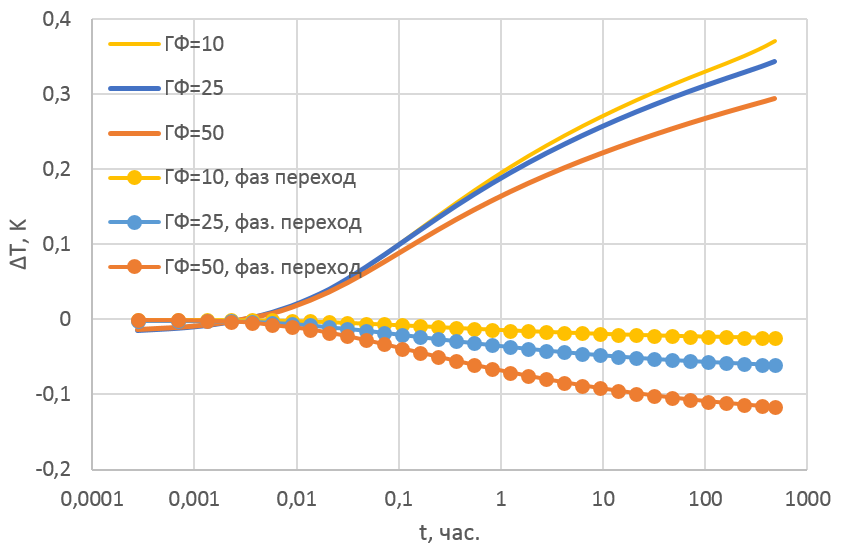
\includegraphics[width=0.8\textwidth]{pic/phase_trans.png}}
	\caption{Влияние поглощения тепла при фазовом переходе на динамику забойной температуры при различных газовых факторах нефти. Запуск скважины с постоянной депрессией.}
	\label{pic:phase_trans}
\end{figure}
	На Рис. \ref{pic:phase_trans} представлено влияние фазовых переходов на температурную аномалию при различных газовых факторах нефти. Видно, что при $\Gamma > 25$ эффект начинает играть существенную роль.

\subsection{Влияние несовершенста ОЗП на динамику забойной температуры. Определение характеристик ОЗП.}
	
	Перейдём к рассмотрению несовершенств.
	Как было указано выше ФЕС ОЗП претерпевают изменение вследствие различных технологических прцоессов.
	Здесь мы будем рассматривать ухудшенные ФЕС.
	Основной характеристикой данного эффекта является скин-фактор, который определяет дополнительное гидродинамическое сопротивление, которое получает пласт из-за этого несовершенства.
\begin{figure}[H]
	\begin{subfigure}[b]{0.5\textwidth}
	\centering
	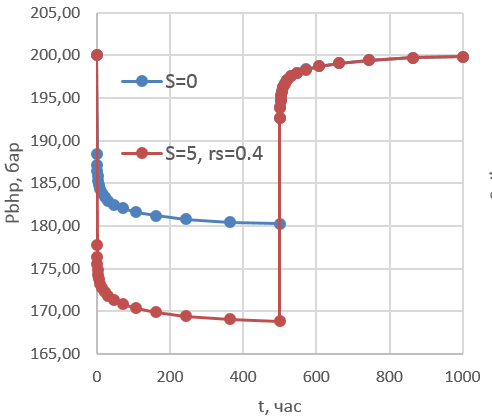
\includegraphics[width=0.9\textwidth]{pic/pres_fes.png}
	\caption{Динамика забойного давления.}
	\label{pic:pres_fes}
	\end{subfigure}
~
	\begin{subfigure}[b]{0.5\textwidth}
		\centering
		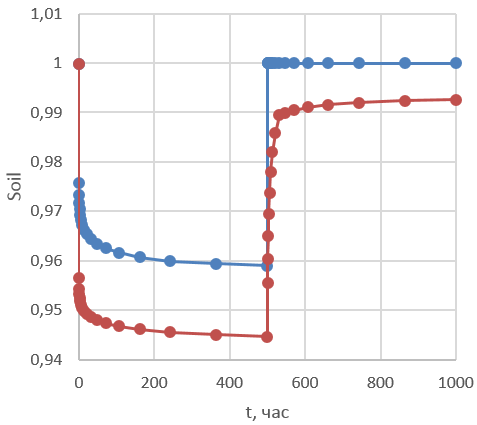
\includegraphics[width=0.9\textwidth]{pic/sat_fes.png}
		\caption{Динамика забойной нефтенасыщенности.}
		\label{pic:sat_fes}
	\end{subfigure}
	\begin{subfigure}[b]{0.5\textwidth}
		\centering
		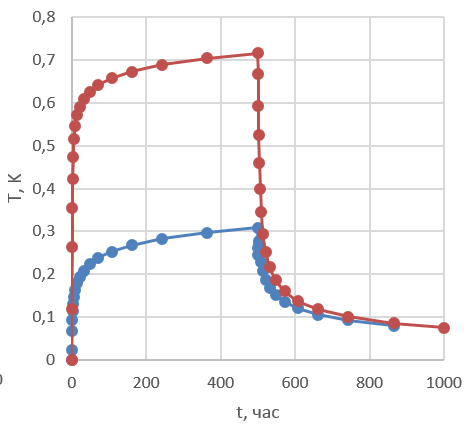
\includegraphics[width=0.9\textwidth]{pic/temp_fes.png}
		\caption{Динамика забойной температуры.}
		\label{pic:temp_fes}
	\end{subfigure}
	\caption{Влияние ухудшенных ФЕС ОЗП на динамику различных величин. Запуск с постоянной депрессией, затем остановка на КВД. Скин ОЗП $S=5$, размер ОЗП -- $r_s=0.4 \text{м}$.}
	\label{pic:fes}
\end{figure}

	На Рис. \ref{pic:fes} представлено влияние ухудшенных ФЕС по сравнению с ФЕС пласта. Из графиков видно влияние данного несовершенства на динамику давления, нефтенасыщенности и температуры.
	Очевидно, что температурная аномалия вызванная данным несовершенством прямо пропорциональна его степени, или же скин-фактору.

	На Рис. \ref{pic:sens_fes} проиллюстрирован факт чувствительности забойной температуры к параметрам ОЗП (размеру проницаемости), нечувствительности давления. Путём адаптации свойств ОЗП к промысловым данным можно найти эти свойства.
	
\begin{figure}[H]
	\begin{subfigure}[b]{0.5\textwidth}
	\centering
	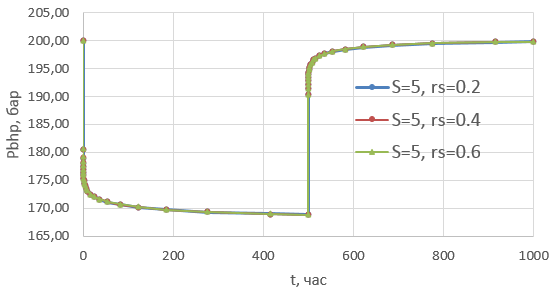
\includegraphics[width=1\textwidth]{pic/pres_sens.png}
	\caption{График давления при различных размерах ОЗП.}
	\label{pic:pres_sens}
	\end{subfigure}
~
	\begin{subfigure}[b]{0.5\textwidth}
		\centering
		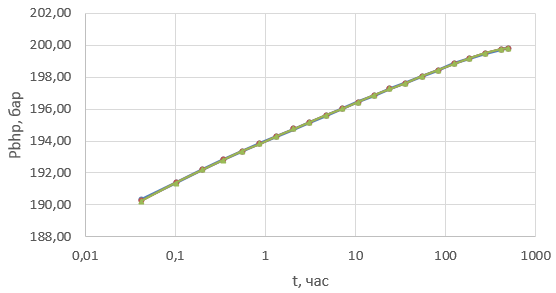
\includegraphics[width=1\textwidth]{pic/pres_sens1.png}
		\caption{КВД. Отсутствие какой-либо чувствительности к размеру ОЗП.}
		\label{pic:pres_sens1}
	\end{subfigure}
	\begin{subfigure}[b]{0.5\textwidth}
		\centering
		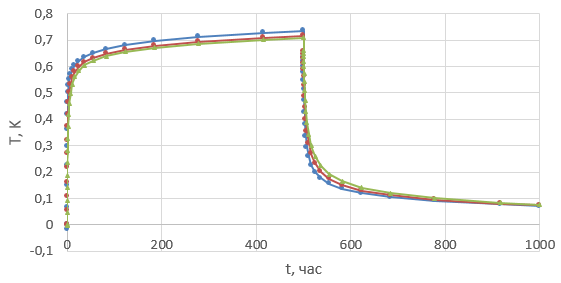
\includegraphics[width=1\textwidth]{pic/temp_sens.png}
		\caption{График температуры при различных размерах ОЗП.}
		\label{pic:temp_sens}
	\end{subfigure}
~
	\begin{subfigure}[b]{0.5\textwidth}
		\centering
		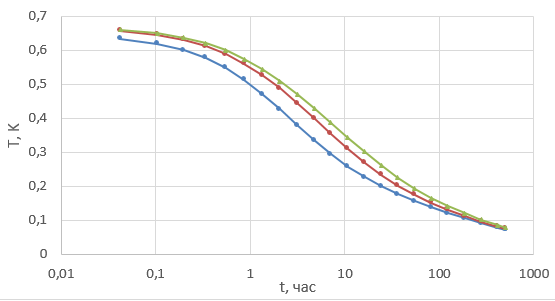
\includegraphics[width=1\textwidth]{pic/temp_sens1.png}
		\caption{Восстановление температуры. Видна чувствительность к размеру ОЗП.}
		\label{pic:temp_sens1}
	\end{subfigure}
	\caption{Чувствительность давления и температуры к изменению размера ОЗП.}
	\label{pic:sens_fes}
\end{figure}

	На Рис. \ref{pic:h} представлен анализ чувствительности модели к параметрам ОЗП при частичном вскрытии скважины для различных размеров пласта, когда течение перестаёт быть одномерным.
	Из графиков можно проследить время термозондирования кровли/подошвы, его изменение для различных мощностей. Также можно отметить размыв границы ОЗП при увеличении размеров ОЗП, как следствие -- уменьшение точности метода.
\begin{figure}[H]
	\begin{subfigure}[b]{0.5\textwidth}
	\centering
	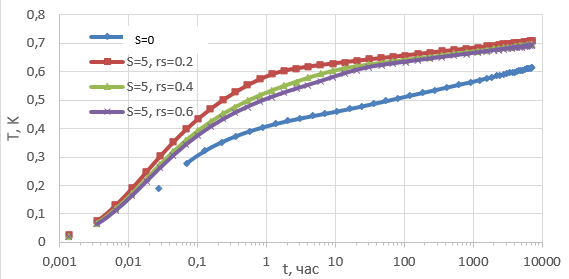
\includegraphics[width=1\textwidth]{pic/h01.png}
	\caption{Сравнение для пласта мощностью $h=0.1\text{м}$.}
	\label{pic:h01}
	\end{subfigure}
~
	\begin{subfigure}[b]{0.5\textwidth}
		\centering
		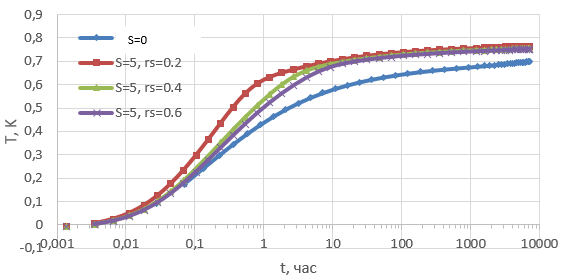
\includegraphics[width=1\textwidth]{pic/h1.png}
	\caption{Сравнение для пласта мощностью $h=1\text{м}$.}
	\label{pic:h1}
	\end{subfigure}
	\begin{subfigure}[b]{0.5\textwidth}
		\centering
		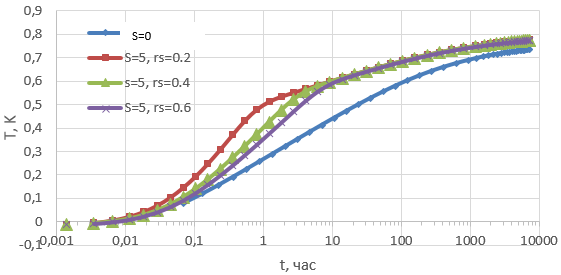
\includegraphics[width=1\textwidth]{pic/h10.png}
		\caption{Сравнение для пласта мощностью $h=10\text{м}$.}
		\label{pic:h10}
	\end{subfigure}
	\caption{Анализ чувствительности модели к параметрам ОЗП при частичном вскрытии скважины для различных размеров пласта.}
	\label{pic:h}
\end{figure}

	На Рис. \ref{pic:adapt} проиллюстрирована совместная интерпретация забойных давления и температуры, полученных с одного из месторождений Западной Сибири.
	Динамика давления воспроизведена по результатам интерпретации ГДИ.
	Затем были подобраны пареметры термодинамической модели, произведена интерпретация ТГДИ, получены характеристики ОЗП: $S = 5.6$, $r_s = 1.2 \text{м}$, $k_s = 102.3 \text{мД}$ при проницаемости пласта $k = 380 \text{мД}$.
	При адаптации использовалась модель двухфазной неизотермической фильтрации с фазовыми переходами.
	Сама адаптация производилась из условия лучшего совпадения (best matching) кривых, с последовательным приближением различных параметров.

\begin{figure}[H]
	\begin{subfigure}[b]{0.5\textwidth}
	\centering
	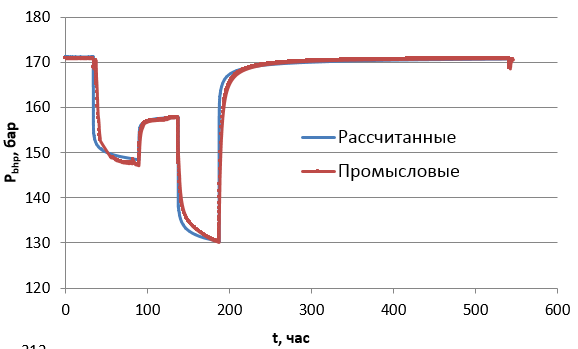
\includegraphics[width=1\textwidth]{pic/adapt_pres.png}
	\caption{Адаптация забойного давления на основе результатов ГДИ.}
	\label{pic:adapt_pres}
	\end{subfigure}
~
	\begin{subfigure}[b]{0.5\textwidth}
		\centering
		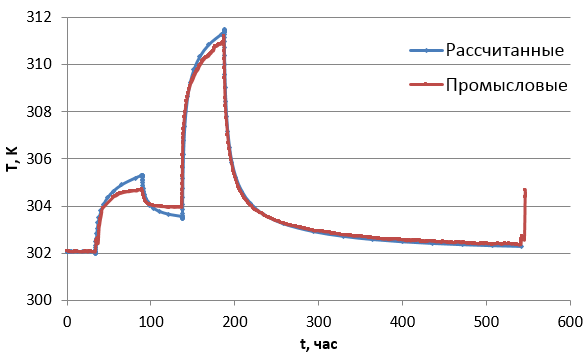
\includegraphics[width=1\textwidth]{pic/adapt_temp.png}
		\caption{Адаптация забойной температуры к используемой модели.}
		\label{pic:adapt_temp}
	\end{subfigure}
	\begin{subfigure}[b]{0.5\textwidth}
		\centering
		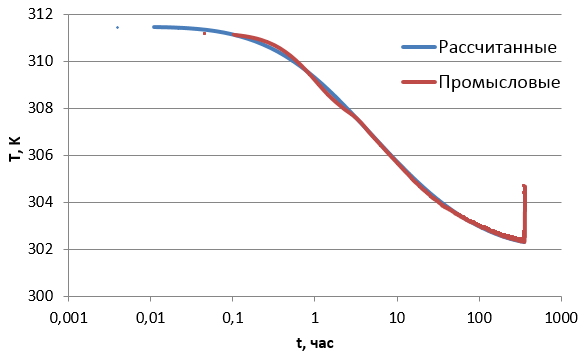
\includegraphics[width=1\textwidth]{pic/adapt_temp1.png}
		\caption{Кривая восстановления температуры.}
		\label{pic:adapt_temp1}
	\end{subfigure}
	\caption{Пример интерпретации скважинных данных на основе разработанной методики.}
	\label{pic:adapt}
\end{figure}

\subsection{Влияние вторичного вскрытия на динамику забойной температуры.}
	Каналы задавались специальными вырезами в сетке. При расчётах распределения дебита считалось что каналы имеют бесконечную проводимость (как и ствол).
	
	На Рис. \ref{pic:grid} представлены внешний вид сетки в прискважинной области и непосредственно каналы внутри сетки.
	
	На Рис. \ref{pic:tunnels} представлена динамика забойной температуры для каналов различной длины.
	Проиллюстрирована температурная аномалия во времени на трёх вежимах добычи: $p_w=180\,\text{бар}$, $p_w=140\,\text{бар}$, $p_w=100\,\text{бар}$ при пластовом давлении $p_e=200\,\text{бар}$. Длина каналов задана
	количеством вырезанных ячеек.
	Каналы, как и следовало ожидать, уменьшают температурную аномалию, т.к. снижают гидродинамическое сопротивление среды.

	На Рис. \ref{pic:tun_fes} изображена постановка задачи притока жидкости к перфорационным каналам при существующей ОЗП с пониженными ФЕС.
	При этом каналы прошивают ОЗП, и приток сосредотачивается именно в эимх местах.
	Это проиллюстрировано на Рис. \ref{pic:tunnels-top1}, где показан вид каналов в трёх измерениях, а также поле скоростей нефти. На Рис. \ref{pic:tunnels-fes} показано то же самое, только в двух измерениях -- на срезе срединной плоскости пласта (совпадает с плоскостью где лежат все каналы).
	
\begin{figure}[H]
	\begin{subfigure}[b]{0.5\textwidth}
	\centering
	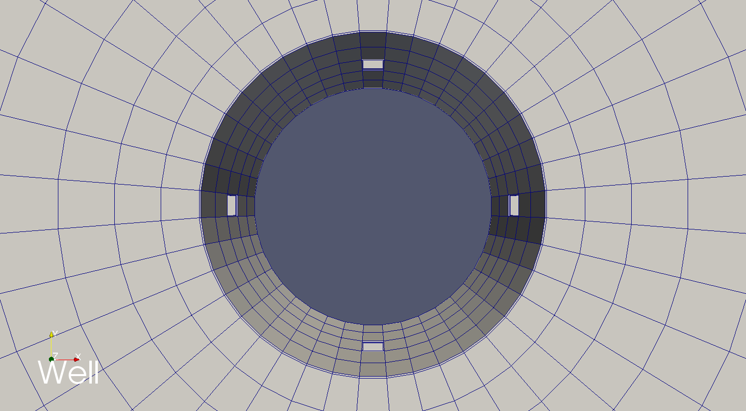
\includegraphics[width=1\textwidth]{pic/grid-top.png}
	\label{pic:grid-top}
	\end{subfigure}
~
	\begin{subfigure}[b]{0.5\textwidth}
		\centering
		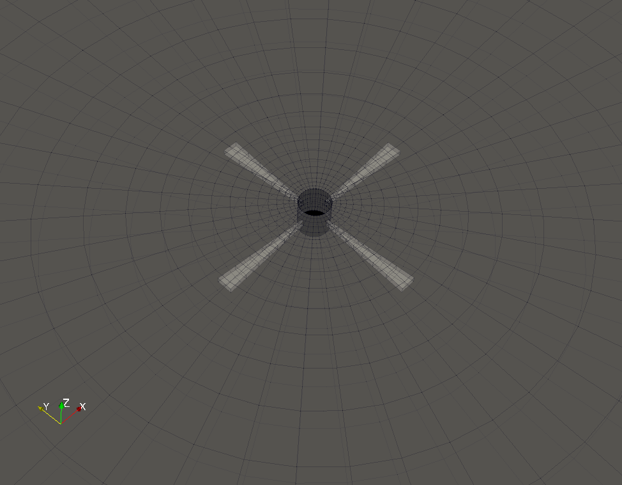
\includegraphics[width=1\textwidth]{pic/tunnels-top.png}
		\label{pic:tunnels-top}
	\end{subfigure}

	\caption{Внешний вид расчётной сетки и каналов.}
	\label{pic:grid}
\end{figure}

\begin{figure}[H]
	\begin{subfigure}[b]{0.5\textwidth}
	\centering
	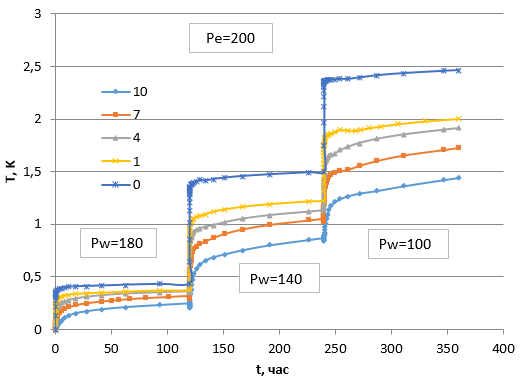
\includegraphics[width=1\textwidth]{pic/temp_tunnels.png}
	\label{pic:temp-tunnels}
	\caption{Динамика забойной температуры во времени для различных длин каналов на трёх режимах: $p_w=180\,\text{бар}$, $p_w=140\,\text{бар}$, $p_w=100\,\text{бар}$ при пластовом давлении $p_e=200\,\text{бар}$.}
	\end{subfigure}
~
	\begin{subfigure}[b]{0.5\textwidth}
		\centering
		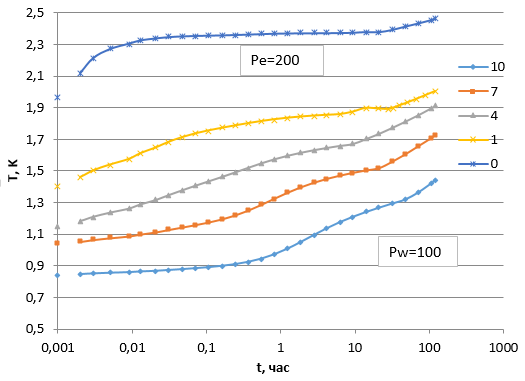
\includegraphics[width=1\textwidth]{pic/temp_tunnels1.png}
		\label{pic:temp-tunnels1}
		\caption{Динамика забойной температуры во времени для различных длин каналов на режиме $p_w=100\,\text{бар}$ при пластовом давлении $p_e=200\,\text{бар}$.}
	\end{subfigure}

	\caption{Динамика забойной температуры на трёх режимах для каналов различной длины (длина -- количество вырезанных ячеек).}
	\label{pic:tunnels}
\end{figure}

	На Рис. \ref{pic:tunnelss} представлена динамика забойной температуры для каналов различной длины и различных размерах ОЗП.
	Видно почти полнёшее сходство графиков без изменённых ФЕС ОЗП и графиков с каналами прошивающими ОЗП. 
	Следовательно, в случае, когда каналы прошивают ОЗП динамика температуры не информативна относительно характеристик ОЗП.
	

\begin{figure}[H]
	\begin{subfigure}[b]{0.5\textwidth}
	\centering
	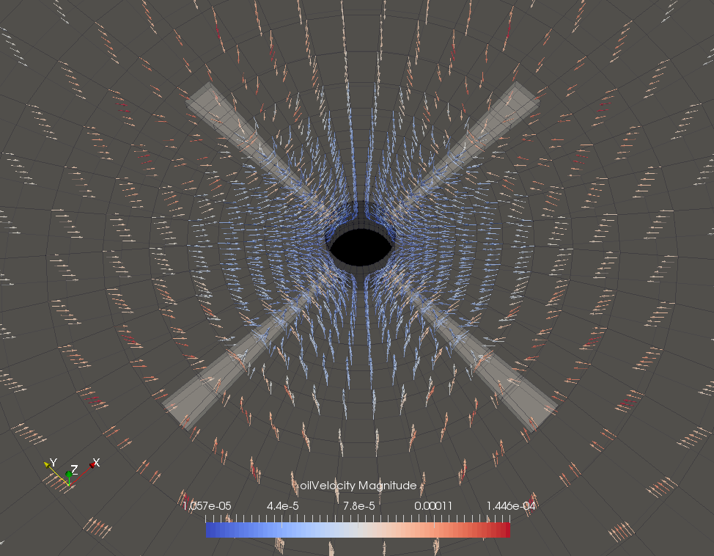
\includegraphics[width=1\textwidth]{pic/tunnels-top1.png}
	\caption{Поле скоростей притока нефти к каналам прошивающим ОЗП.}
	\label{pic:tunnels-top1}
	\end{subfigure}
~
	\begin{subfigure}[b]{0.5\textwidth}
		\centering
		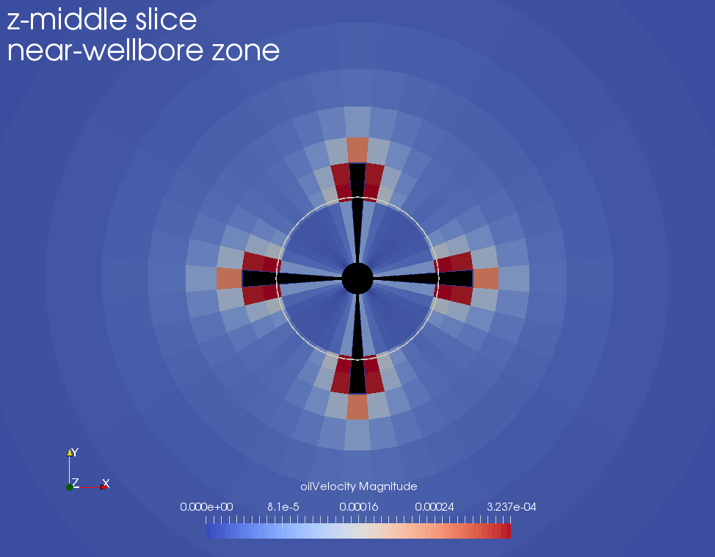
\includegraphics[width=1\textwidth]{pic/tunnels-fes.png}
		\caption{Амплитуда скорости фильтрации нефти при притоке к каналам.}
		\label{pic:tunnels-fes}
	\end{subfigure}

	\caption{Вид притока к каналам с ухудшенными ФЕС ОЗП, прошивающим ОЗП.}
	\label{pic:tun_fes}
\end{figure}

\begin{figure}[H]
	\begin{subfigure}[b]{0.5\textwidth}
	\centering
	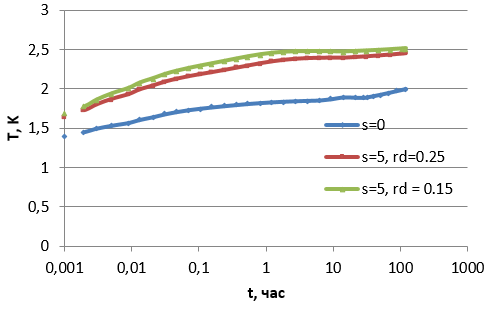
\includegraphics[width=1\textwidth]{pic/tunnels1.png}
	\caption{Температура на режиме, приток к каналам длины 1. Каналы не прошивают ОЗП.}
	\label{pic:tunnels1}
	\end{subfigure}
~
	\begin{subfigure}[b]{0.5\textwidth}
		\centering
		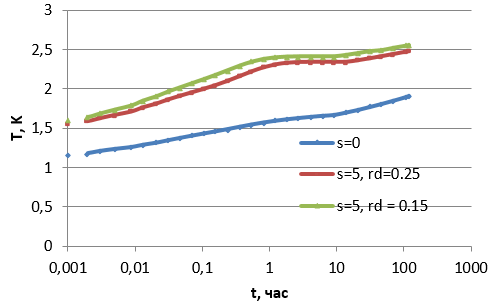
\includegraphics[width=1\textwidth]{pic/tunnels4.png}
		\caption{Температура на режиме, приток к каналам длины 4. Каналы не прошивают ОЗП.}
		\label{pic:tunnels4}
	\end{subfigure}
	\begin{subfigure}[b]{0.5\textwidth}
	\centering
	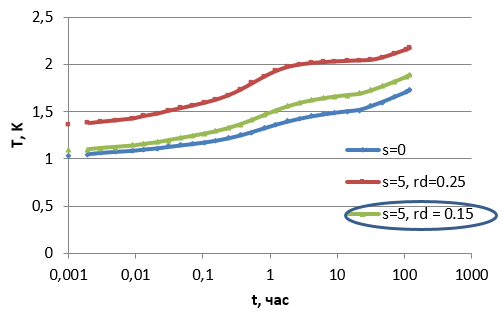
\includegraphics[width=1\textwidth]{pic/tunnels7.png}
	\caption{Температура на режиме, приток к каналам длины 7. Для одного случая каналы прошили ОЗП.}
	\label{pic:tunnels7}
	\end{subfigure}
~
	\begin{subfigure}[b]{0.5\textwidth}
		\centering
		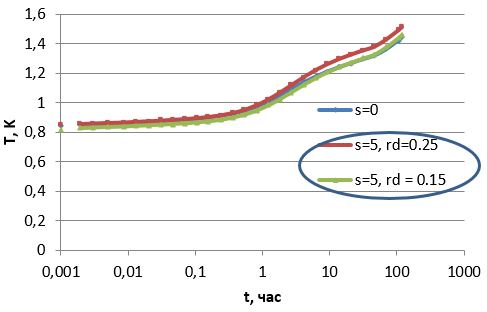
\includegraphics[width=1\textwidth]{pic/tunnels10.png}
		\caption{Температура на режиме, приток к каналам длины 10. Каналы прошили ОЗП в двух постановках.}
		\label{pic:tunnels10}
	\end{subfigure}

	\caption{Динамика температуры на забое для различных длин каналов, размеров ОЗП.}
	\label{pic:tunnelss}
\end{figure}

